\documentclass[lerntheke,12pt,a5paper,landscape]{arbeitsblatt}

\ladeModule{theme}

\ladeFach[quelltexte]{informatik}

\aboptionen{
	name		= {J. Neugebauer},
	kuerzel 	= {Ngb},
	titel 		= {Lerntheke Webseiten erstellen mit HTML},
	reihe 		= {Webseiten erstellen mit HTML},
	fach 		= {Informatik},
	kurs 		= {9Diff},
	nummer 		= {2},
	lizenz 		= {cc-by-nc-sa-eu-4},
	version 	= {2022-09-21},
	%seitenzahlen= {keine},
}

\setminted{linenos=false}

\begin{document}



\begin{hilfekarte}{CSS-Regeln}{hilfe:regeln}
	\hilfeMarke{hilfe:vererbung}
	Eine \emph{CSS-Regel} wird im Format \mintinline{css}{css-eigenschaft: wert;} verfasst.

	Die \emph{CSS-Eigenschaft} bestimmt, welcher Teil des HTML-Elements verändert werden soll. Es gibt eine große Liste an CSS-Eigenschaften, wie
	\begin{smallitem}
		\item \code{color}
		\item \code{background-color}
		\item \code{font-family}
		\item \code{border}
		\item uvm.
	\end{smallitem}

	Je nach \emph{CSS-Eigenschaft} sind andere Werte erlaubt.
\end{hilfekarte}

\begin{loesungskarte}[CSS-Regeln]
	Um eine \emph{CSS-Regel} auf ein \emph{HTML-Tag} anzuwenden, kann dem Tag ein Attribut mit dem Namen \code{style} hinzugefügt werden.

	\begin{minted}{HTML}
	<h1 style="color:#FF0000;font-weight:600;">Meine Überschrift</h1>
	<p style="font-family:Arial;text-decoration:underline;">Text text text ...</p>
	\end{minted}
\end{loesungskarte}

\begin{hilfekarte}{Definition von Farben}{hilfe:farben}
	Farben können in CSS-Regeln auf verschiedene Weisen angegeben werden. Am häufigsten werden sie im RGB-Farbraum definiert. RGB steht für \textbf{R}ot, \textbf{G}rün und \textbf{B}lau und beschreibt eine Farbe durch die enthaltenen Anteile dieser drei Farben.

	Es gibt verschiedene Arten, diese drei Anteile zu beschreiben. Im Web ist es üblich, die Farben als ganze Zahlen zwischen \code{0} und \code{255} oder als entsprechende Hexadezimalzahl (\code{00} bis \code{FF}) anzugeben.

	\begin{center}
		\colorbox[RGB]{102,214,26}{R: 102 G: 214 B: 26} \qquad \colorbox[RGB]{200,30,80}{\textcolor{white}{R: 200 G: 30 B: 80}} \qquad \colorbox[RGB]{50,98,200}{\textcolor{white}{R: 50 G: 98 B: 200}}
	\end{center}

	In einer CSS-Anweisung kann eine RGB-Farbe direkt oder im Hexadezimal-Format angegeben werden:
	\begin{minted}{CSS}
	background-color: rgb(102,214,26);
	color: #C81E50;
	\end{minted}

	Unter \url{https://link.ngb.schule/farbmischer} findest Du einen Farbmischer, um eigene Farben zu mischen.
\end{hilfekarte}

\begin{loesungskarte}[Definition von Farben]
	CSS kennt auch einige Farben bei Namen:
	\begin{minted}{CSS}
	background-color: white;
	color: black;
	border-color: cyan;
	\end{minted}

	Eine Liste der Farbnamen findest Du unter \url{https://link.ngb.schule/farbnamen}.

	Namen der Grundfarben:
	\begin{tasks}[label=](5)
		\task \code{white}
		\task \code{yellow}
		\task \code{fuchsia}
		\task \code{red}
		\task \code{silver}
		\task \code{gray}
		\task \code{olive}
		\task \code{purple}
		\task \code{maroon}
		\task \code{aqua}
		\task \code{lime}
		\task \code{teal}
		\task \code{green}
		\task \code{blue}
		\task \code{navy}
		\task \code{black}
	\end{tasks}
\end{loesungskarte}

\begin{hilfekarte}{Größenangaben}{hilfe:groessen}
CSS kennt verscheidene Einheiten, um Größenangaben zu machen. Es ist möglich eine Größe in \code{mm} anzugeben, aber da ein Millimeter auf verschiedenen Ausgabegeräten unterschiedlich groß dargestellt wird, benutzt man lieber Einheiten, die \emph{relative} Größen angeben. Auf diese Weise wird eine Überschrift zum Beispiel auf einem Smartphone kleiner angezeigt, als auf einem großen Monitor, aber die Überschrift ist in beiden Fällen größer als der Text.

Häufig verwendete Einheiten sind:
\begin{smalldescr}
	\item[\code{pt}] (\enquote{point}) \code{12pt} ist eine übliche Schriftgröße für Dokumente. Ein Zentimeter entspricht etwas \SI{28,4}{pt}. Diese Einheit bietet sich für Schriftgrößen an.
	\item[\code{px}] (\enquote{pixel}) Mit Pixeln wird Elementen eine feste Größe zugewiesen. Diese Einheit bietet sich für die Dicke von Rahmenlinien oder Größenangaben von Bildern an.
	\item[\code{em}] Relative Einheit, die abhängig von der Schriftgröße ist. Die Einstellung \SI{1.2}{em} stellt den Text also etwas größer dar, als die normale Schriftgröße. \SI{0.8}{em} ist etwas kleiner. Diese Einheit bietet sich für relative Schriftgrößen (Überschriften, Fußnoten) oder Abstände an (z.B. zwischen Absätzen), die abhängig von der Schriftgröße mitwachen / schrumpfen sollen.
\end{smalldescr}
\end{hilfekarte}

\leereKarte

\begin{hilfekarte}{Vererbung von CSS-Regeln}{hilfe:vererbung}
	CSS-Regeln werden \enquote{vererbt}. Das bedeutet, wenn du einem HTML-Tag eine CSS-Regel hinzufügst, dann wird diese Regel in der Regel auch auf HTML-Tags angewandt, die sich \emph{innerhalb} dieses Tags befinden.

	Im Beispiel auf der Rückseite wurde dem \code{body}-Tag eine CSS-Regel hinzugefügt, die die Textfarbe auf Rot setzt. Diese Regel wird an das \code{h1}- und das \code{p}-Tag weitervererbt. Und das \code{p}-Tag vererbt die Eigenschaft wiederum an das innenliegende \code{strong} und \code{em} weiter.

	\begin{center}
	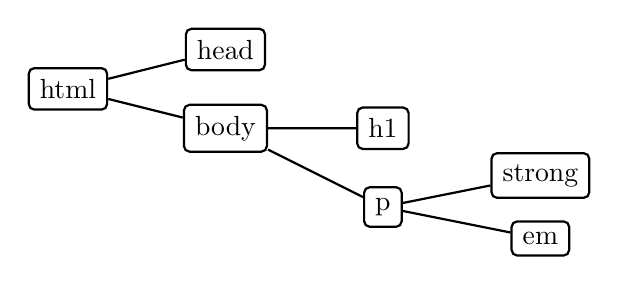
\begin{tikzpicture}[tag/.style={draw,thick,inner sep=4px,rounded corners=2px}]
		\node[tag] (HTML) at (0,0) {\code{html}};
			\node[tag] (HEAD) at (2,0.5) {\code{head}};
			\node[tag] (BODY) at (2,-0.5) {\code{body}};
				\node[tag] (H1) at (4,-0.5) {\code{h1}};
				\node[tag] (P) at (4,-1.5) {\code{p}};
					\node[tag] (STRONG) at (6,-1.1) {\code{strong}};
					\node[tag] (EM) at (6,-1.9) {\code{em}};
		\draw[thick] (HTML) -- (HEAD);
		\draw[thick] (HTML) -- (BODY) -- (H1);
		\draw[thick] (BODY) -- (P) -- (STRONG);
		\draw[thick] (P) -- (EM);
	\end{tikzpicture}
	\end{center}

	Das \code{strong}-Tag definiert allerdings eine eigene Schriftfarbe und überschreibt somit die vererbte Regel.

	Das \code{p}-Tag definiert wiederum eine Regel, die den Text unterstreicht. Somit iwird diese Regel auch an \code{strong} und \code{em} vererbt (aber nicht an \code{h1}, da die Überschrift nicht \enquote{innerhalb} des \code{p} liegt). \code{em} definiert sich aber wieder eine eigene \code{text-decoration} und entfernt die geerbte Unterstreichung.
\end{hilfekarte}

\begin{loesungskarte}[Vererbung von CSS-Regeln]
	\begin{minted}{HTML}
		<html>
		<head>
			<title>Testseite</title>
		</head>
		<body style="color:red;">
			<h1>Meine Testseite</h1>
			<p style="text-decoration:underline;">Weit hinten, hinter den
			Wortbergen, fern der Länder Vokalien und Konsonantien leben die
			<strong style="color:blue;">Blindtexte</strong>. Abgeschieden
			wohnen sie in <em style="text-decoration:normal;">Buchstabenhausen</em>
			an der Küste des Semantik, eines großen Sprachozeans.</p>
		</body>
		</html>
	\end{minted}
\end{loesungskarte}




\begin{karte1}{Hintergrundfarbe}
	\hilfeMarke{hilfe:farben}\hilfeMarke{hilfe:regeln}
	Du kannst die Hintergrundfarbe von Elementen verändern, indem Du dem Tag eine CSS-Regel mit der Eigenschaft \code{background-color} hinzufügst.

	\begin{minted}{CSS}
	background-color: Farbe;
	\end{minted}

	Beispiel:
	\begin{minted}{html}
	<h1 style="background-color:#FF0000;">Meine Überschrift</h1>
	\end{minted}

	Um den Hintergrund der kompletten Seite zu verändern, musst Du die CSS-Regel dem \code{body}-Tag hinzufügen.

	\begin{minted}{html}
	<body style="background-color:rgb(255, 0, 0);">
	\end{minted}
\end{karte1}

\leereKarte

\begin{karte1}{Schriftarten}
	\hilfeMarke{hilfe:regeln}\hilfeMarke{hilfe:groessen}
	Du kannst die Schriftart eines Elements verändern, indem Du dem Element eine CSS-Regel mit der Eigenschaft \code{font-family} hinzufügst. Die Größe der Schrift kannst Du mit der Eigenschaft \code{font-size} beeinflussen.

	\begin{minted}{CSS}
		font-family: Schriftart, Alternative Schriftart;
		font-size: Schriftgröße;
	\end{minted}

	Beispiel:
	\begin{minted}{html}
	<h1 style="font-family:Arial, Helvetica;font-size:20pt;">Meine Überschrift</h1>
	\end{minted}

	Um die Schriftart der kompletten Seite zu verändern, musst Du die CSS-Regel dem \code{body}-Tag hinzufügen.

	\begin{minted}{html}
	<body style="font-family:'Brush Script MT';">
	\end{minted}
\end{karte1}

\begin{loesungskarte}{Schriftarten}
	Nicht jede Schriftart ist auf jedem Endgerät verfügbar. Besondere Schirftarten (Schreibschriften, ...) solltest Du im Web vermeiden, denn sie sind unter Umständen schwer lesbar. Vor allem auf Mobilgeräten...

	Die folgende Liste von Schriftarten, die auf jedem Gerät funktionieren sollten, findest du unter \url{https://link.ngb.schule/html-fonts}.

	\begin{smallitem}
		\item Arial (sans-serif)
		\item Verdana (sans-serif)
		\item Tahoma (sans-serif)
		\item Trebuchet MS (sans-serif)
		\item Times New Roman (serif)
		\item Georgia (serif)
		\item Garamond (serif)
		\item Courier New (monospace)
		\item Brush Script MT (cursive)
	\end{smallitem}
\end{loesungskarte}

\begin{karte2}{Textauszeichnungen}
	\hilfeMarke{hilfe:regeln}
	Du kennst schon einnige HTML-Tags, mit denen du Textstellen besonders kennzeichnen kannst (z.B. \code{<strong> ... </strong>} für Fettdruck). Diese Effekte kannst du auch für ganze Elemente mit einer CSS-Eigenschaft definieren.

	\begin{description}
		\item[\code{font-weight}:] Wie \enquote{fett} der Text sein soll. Mögliche Werte: \code{normal}, \code{bold}, \code{bolder}, \code{lighter}.
		\item[\code{font-style}:] Kursiver Text. Mögliche Werte: \code{normal}, \code{italic}
		\item[\code{text-decoration}:] Unterstreichungen. Mögliche Werte: \code{underline}, \code{overline}, \code{line-through}

		Es dürfen auch mehrere \enquote{Dekorationen} auf einmal verwendet werden und es können Eigenschaften für Rahmenlinien angehängt werden (siehe \prettyref{karte:linien}).
		\begin{minted}{CSS}
			text-decoration: underline overline dotted red;
		\end{minted}
	\end{description}

	Nicht jede Schriftart unterstützt jede der obigen Eigenschaften.
\end{karte2}

\leereKarte

\begin{karte1}{Schriftfarbe}
	\hilfeMarke{hilfe:regeln}\hilfeMarke{hilfe:farben}
	Du kannst die Farbe des Textes verändern, indem Du dem Element eine CSS-Regel mit der Eigenschaft \code{color} hinzufügst.

	\begin{minted}{CSS}
		color: Farbe;
	\end{minted}

	Beispiel:
	\begin{minted}{html}
	<p style="color:blue;">Mein Text</p>
	\end{minted}

	Um die Schriftart der kompletten Seite zu verändern, musst Du die CSS-Regel dem \code{body}-Tag hinzufügen.

	\begin{minted}{html}
	<body style="color:red;">
	\end{minted}
\end{karte1}

\leereKarte

\begin{karte2}{Rahmenlinien}
	\label{karte:linien}
	\hilfeMarke{hilfe:regeln}\hilfeMarke{hilfe:farben}\hilfeMarke{hilfe:groessen}
	Du kannst die Eigenschaften von Rahmenlinien (Tabellen, Textauszeichnungen) mit den \code{border-} Eigenschaften verändern.

	\begin{minted}{CSS}
		border-color: Farbe;
		border-width: Größe;
		border-style: Stil;
	\end{minted}

	Der Rahmenstil kann einen der folgenden Werte annehmen: \code{none}, \code{dotted}, \code{dashed}, \code{solid}, \code{double}, \code{groove}, \code{ridge}, \code{inset}, \code{outset}

	Beispiel:
	\begin{minted}{html}
	<table style="border-color:gray;border-width:4px;border-style:dashed;">
		...
	</table>
	\end{minted}
\end{karte2}

\begin{loesungskarte}{Lösung 5}
	Die \code{border-}Eigenschaften ändern den ganzen Rahmen (oben, unten, rechts und links). Um nur eine der vier Richtungen zu ändern, kannst Du hinter \code{border-} die entsprechende Richtung angeben:

	\begin{minted}{CSS}
		border-top-width: Größe;
		border-bottom-style: Stil;
		border-left-color: Farbe;
		border-right: Größe Stil Farbe;
	\end{minted}

	Die letzte CSS-Regel für die rechte Rahmenlinie ist eine Kurzform, in der Du alle drei Eigenschaften in nur einer Regel verändern kannst. Um den kompletten Rahmen also mit einer roten, gepunktetetn Linie der Dicke 2px zu umgeben, kannst du schreiben:

	\begin{minted}{CSS}
		border-right: 2px dotted red;
	\end{minted}

	{\small\textbf{Tipp}: Du kannst mit \code{border-bottom} zum Beispiel auch einer Überschrift eine besondere Unterstreichung geben.}
\end{loesungskarte}

\begin{karte2}{Textausrichtung und -transformation}
	\hilfeMarke{hilfe:regeln}\hilfeMarke{hilfe:farben}
	Wie im Textsatz üblich, kannst Du auch in HTML den Text der Seite beliebig ausrichten. Dazu wird die CSS-Eigenschaft \code{text-align} verwendet.

	\begin{minted}{CSS}
		text-align: Ausrichtung;
	\end{minted}

	Mögliche Werte sind \code{left}, \code{right}, \code{justify} und \code{center}.

	Eine besondere Art der Textauszeichnung ist eine \emph{Texttransformation}. Mit der Eigenschaft \code{text-transform} kannst du den Text beispielsweise in Großbuchstaben oder Kapitälchen umwandeln.

	\begin{minted}{CSS}
		text-transform: Transformation;
	\end{minted}

	Mögliche Werte sind \code{none}, \code{uppercase}, \code{lowercase} und \code{capitalize}.
\end{karte2}

\begin{loesungskarte}{Textschatten}
	\hilfeMarke{hilfe:regeln}\hilfeMarke{hilfe:farben}\hilfeMarke{hilfe:groessen}
	Eine weitere besondere Art der Textauszeichnung ist ein \emph{Textschatten}. Diese Eigenchaft sollte nur sehr spärlich benutzt werden, aber kann ein richtiger Eyecatcher sein.

	\begin{minted}{CSS}
		text-shadow: Größe Größe Größe Farbe;
	\end{minted}

	Um den SChatten zu definieren müssen vier Werte angegeben werden:
	\begin{smallenum}
		\item Die Verschiebung nach rechts/links.
		\item Die Verschiebung nach oben/unten.
		\item Der Grad der Weichzeichnung des Schattens (wie verschwommen er ist).
		\item Die Farbe des Schattens.
	\end{smallenum}

	Zum Beispiel:
	\begin{minted}{HTML}
		<h1 style="text-shadow: 2px 2px 8px #FF0000;">Meine Überschrift</h1>
	\end{minted}
\end{loesungskarte}

\begin{karte2}{Abstände}
	\hilfeMarke{hilfe:regeln}\hilfeMarke{hilfe:groessen}
	Du kannst die ABstände zwischen Elementen und vom Inhalt eines Elements zu seinem Rand definieren. Der Innenabstand wird als \code{padding} definiert. Der Außenabstand (zum nächsten Element) als \code{margin}. Die Abbildung zeigt, wie sich die Größe eines Elements berechnet, wenn beide Abstände und ein Rahmen festgelegt wurden (blau ist der Inhalt).

	\begin{center}
		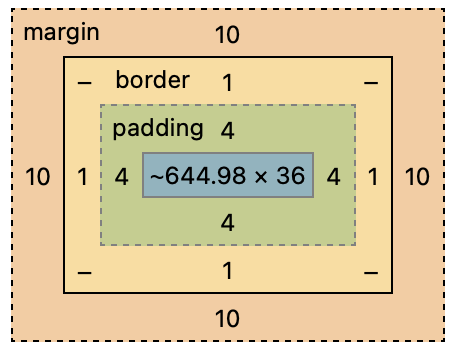
\includegraphics[width=5cm]{9Diff-LT.2-Abb_Abstand.png}
	\end{center}
\end{karte2}

\begin{loesungskarte}[Abstände]
	Um Abstände festzulegen wird entweder die CSS-Eigenschaft \code{margin} bzw. \code{padding} genutzt, die vier Größen als Wert bekommt, für die Abstände oben, rechts, unten und links. Alternativ kann jeder Abstand auch direkt gesetzt werden.
	\begin{minted}{CSS}
		margin: Größe Größe Größe Größe;
		margin-bottom: Größe;
		padding: Größe Größe Größe Größe;
		padding-top: Größe;
	\end{minted}

	Zum Beispiel:
	\begin{minted}{HTML}
		<h1 style="padding-left: 10px;">Meine Überschrift</h1>
		<p style="margin-bottom: 1em;">Mein Text</p>
		<p>Mein Text</p>
	\end{minted}
\end{loesungskarte}

\begin{karte1}{Listen}
	\hilfeMarke{hilfe:regeln}
	Die Art einer Liste kann mit der Eigenschaft \code{list-style-type} festgelegt werden. Es gibt eine ganze Reihe an unterschiedlichen Listenarten. Die Tags \code{ol} und \code{ul} legen automatisch eine Nummerierung mit Zahlen und eine Strichliste fest. Aber beide Listenarten können komplett neu definiert werden.
	\begin{minted}{CSS}
		list-style-type: Listenart;
	\end{minted}

	Mögliche Werte findest Du auf der Rückseite.

	\begin{minted}{HTML}
	<ul style="list-style-type: disc;">
		<li>Eintrag 1</li>
		<li style="list-style-type: lower-roman;">Eintrag 2</li>
	</ul>
	\end{minted}
\end{karte1}

\begin{loesungskarte}[Listen]
	Mögliche Werte für die CSS-Eigenschaft \code{list-style-type}:

	\begin{tasks}[label=](4)
		\task \code{disc}
		\task \code{armenian}
		\task \code{circle}
		\task \code{decimal}
		\task \code{decimal-leading-zero}
		\task \code{georgian}
		\task \code{hebrew}
		\task \code{hiragana}
		\task \code{hiragana-iroha}
		\task \code{katakana}
		\task \code{katakana-iroha}
		\task \code{lower-alpha}
		\task \code{lower-greek}
		\task \code{lower-latin}
		\task \code{lower-roman}
		\task \code{none}
		\task \code{square}
		\task \code{upper-alpha}
		\task \code{upper-greek}
		\task \code{upper-latin}
		\task \code{upper-roman}
	\end{tasks}
\end{loesungskarte}

\begin{karte2}{Mauszeiger}
	\hilfeMarke{hilfe:regeln}
	Mit der CSS-Eigenschaft \code{cursor} kannst du den Mauszeiger verändern, wenn er sich über ein bestimmtes Element bewegt.
	\begin{minted}{CSS}
		cursor: Mauszeiger;
	\end{minted}

	Beispiel:
	\begin{minted}{html}
	<h1 style="cursor:grab;">Meine Überschrift</h1>
	\end{minted}

	Um den Mauszeiger der kompletten Seite zu verändern, musst Du die CSS-Regel dem \code{body}-Tag hinzufügen.

	\begin{minted}{html}
	<body style="cursor:copy;">
	\end{minted}
\end{karte2}

\begin{loesungskarte}[Mauszeiger]
	Mögliche Werte für die CSS-Eigenschaft \code{cursor}:

	\begin{tasks}[label=](5)
		\task\code{alias}
		\task\code{all-scroll}
		\task\code{auto}
		\task\code{cell}
		\task\code{col-resize}
		\task\code{context-menu}
		\task\code{copy}
		\task\code{crosshair}
		\task\code{default}
		\task\code{e-resize}
		\task\code{ew-resize}
		\task\code{grab}
		\task\code{grabbing}
		\task\code{help}
		\task\code{move}
		\task\code{n-resize}
		\task\code{ne-resize}
		\task\code{nesw-resize}
		\task\code{ns-resize}
		\task\code{nw-resize}
		\task\code{nwse-resize}
		\task\code{no-drop}
		\task\code{none}
		\task\code{not-allowed}
		\task\code{pointer}
		\task\code{progress}
		\task\code{row-resize}
		\task\code{s-resize}
		\task\code{se-resize}
		\task\code{sw-resize}
		\task\code{text}
		\task\code{URL}
		\task\code{vertical-text}
		\task\code{w-resize}
		\task\code{wait}
		\task\code{zoom-in}
		\task\code{zoom-out}
	\end{tasks}
\end{loesungskarte}

\begin{karte3}{CSS-Dateien}
	Auf größeren HTML-Seiten mit vielen Tags und CSS-Regeln wird es sehr unübersichtlich, die CSS-Eigenschaften in jedem Tag im \code{style}-Attribut zu notieren. Vor allem, wenn ein Stil für mehrere Elemente benutzt werden soll (zum Beispiel alle \code{em}-Tags auf der ganzen Seite).

	Daher ist es üblich, die CSS-Regeln in einer separaten Datei (z.B. \datei{style.css}) im selben Ordner wie die HTML-Datei zu speichern.

	Der HTML-Seite wird diese Style-Datei mit einem \enquote{Metatag} bekannt gemacht. Das Tag steht innerhalb des \code{head}-Tags der HTML-Seite:
	\begin{minted}{HTML}
	<head>
		<title>Titel der Seite</title>
		<link rel="stylesheet" type="text/css" href="style.css">
	</head>
	\end{minted}

	Innerhalb der CSS-Datei müssen nun alle die CSS-Regeln für ein Element zusammen mit einem \emph{CSS-Selektor} notiert werden, der angibt, für welches Tag dise Regel gedacht ist.
\end{karte3}


\begin{loesungskarte}[CSS-Dateien]
	\begin{links}
		\paragraph{Schema\phantom{p}}
		\begin{minted}{CSS}
		selektor {
			eigenschaft1: wert1;
			eigenschaft2: wert2;
		}
		\end{minted}
	\end{links}\begin{rechts}
		\paragraph{Beispiel}
		\begin{minted}{CSS}
		p {
			color: #ae34f2;
			text-decoration: underline;
		}
		\end{minted}
	\end{rechts}

	\vspace*{1.2em}
	\begin{links}
		Ein CSS-Selektor kann aus einem oder mehreren HTML-Tags bestehen:
		\begin{minted}{CSS}
		p { }
		h1, h2, h3, h4, h5, h6 { }
		em, strong { }
		\end{minted}
	\end{links}\begin{rechts}
		Außerdem kann ein Selektor aus einer \emph{CSS-Klasse} bestehen. Dazu beginnt der Selektor mit einem Punkt:
		\begin{minted}{CSS}
			.roter-text { }
		\end{minted}
		In der HTML-Datei muss die Klasse dann mit dem \code{class}-Attribut einem Tag zugewiesen werden:
		\begin{minted}{CSS}
			<p class="roter-text">...</p>
		\end{minted}
	\end{rechts}
\end{loesungskarte}

\end{document}
